\chapter{Specifikacija programske potpore}
	
	\section{Funkcionalni zahtjevi}
	
	
	\noindent \textbf{Dionici:}
	
	\begin{packed_enum}
		
		\item Administrator-voditelj tima
		\item Razvojni tim CodeCooks			
		\item Profesori predmeta Programsko inžinjerstvo
		\item Korisnici
		
	\end{packed_enum}
	
	\noindent \textbf{Aktori i njihovi funkcionalni zahtjevi:}
	
	
	\begin{packed_enum}
		\item  \underbar{Admin može:}
		
		\begin{packed_enum}
			
			\item Upravljanje korisnicima
			\item Upravljanje receptima
			\begin{packed_enum}
				
				\item  Brisanje recepata
				\item  Uređivanje recepata
				
			\end{packed_enum}
			\item Upravljanje komentarima
			\begin{packed_enum}
				
				\item  Brisanje komentara 
				\item  Cenzuriranje komentara
				
			\end{packed_enum}
			\item  Mjenjanje kategorija
			
		\end{packed_enum}
		
		\item  \underbar{Registrirani korisnik može:}
		
		\begin{packed_enum}
			
			\item Objavljivanje recepata
			\item Komuniciranje s ostalim registriranim korisnicima
			\item Objavljivanje termina za komunikaciju
			\item Označavanje recepata
			\item Komentiranje recepata
			\item Spremanje recepata
			\item Praćenje drugih registriranih korisnika
			\item Upravljanje dozvolama pratiteljima
			\item Upravljanje osobnim informacijama
			\item Upravljanje postavkama komunikacije i obavijestima
			
		\end{packed_enum}
		
		\item  \underbar{Neregistrirani korisnik može:}
		
		\begin{packed_enum}
			
			\item Pregledavanje recepata temeljem kategorija
			
		\end{packed_enum}
		
		
		\item  \underbar{Baza podataka može:}
		
		\begin{packed_enum}
			
			\item Pohrana osobnih podataka registriranog korisnika
			\item Pohrana recepata
			\item Pohrana komentara
			
		\end{packed_enum}
	\end{packed_enum}
	
	\eject 
	
	
	\noindent \underbar{\textbf{UC1 - Pregled recepata}}
	\begin{packed_item}
		
		\item \textbf{Glavni sudionik: Neregistrirani korisnik, Registrirani korisnik}
		\item  \textbf{Cilj: Pregled recepata temeljem kategorija} 
		\item  \textbf{Sudionici: Baza podataka} 
		\item  \textbf{Preduvjet: -} 
		\item  \textbf{Opis osnovnog tijeka:}
		
		\item[] \begin{packed_enum}
			
			\item Korisnik otvori platformu
			\item Ponuđene su mu kategorije, vrste kuhinje, specifični sastojci
			\item Korisnik odabire što želi i prikazuju mu se recepti
		\end{packed_enum}
		
	\end{packed_item}
	
	
	\noindent \underbar{\textbf{UC2 - Registracija}}
	\begin{packed_item}
		
		\item \textbf{Glavni sudionik: Neregistrirani korisnik}
		\item  \textbf{Cilj: Stvaranje računa za pristup ostalim značajkama sustava}  
		\item  \textbf{Sudionici: Baza podataka} 
		\item  \textbf{Preduvjet:-} 
		\item  \textbf{Opis osnovnog tijeka:}
		
		\item[] \begin{packed_enum}
			
			\item Korisnik odabire opciju za registraciju
			\item Korisnik unosi potrebne korisničke podatke
			\item Korisnik prima obavijest o uspješnoj registraciji
		\end{packed_enum}
		
		\item  \textbf{Opis mogućih odstupanja:}
		
		\item[] \begin{packed_item}
			
			\item[2.a] Odabir već zauzetog korisničkog imena i/ili e-maila, unos korisničkog podatka u nedozvoljenom formatu ili pružanje neispravnoga e-maila
			\item[] \begin{packed_enum}
				
				\item  Sustav obavještava korisnika o neuspjelom upisu i vraća ga na stranicu za registraciju
				\item Korisnik mijenja potrebne podatke te završava unos ili odustaje od registracije
				
			\end{packed_enum}
			
		\end{packed_item}
	\end{packed_item}
	
	
	\noindent \underbar{\textbf{UC3 - Prijava u sustav}}
	\begin{packed_item}
		
		\item \textbf{Glavni sudionik: }
		\item  \textbf{Cilj: Dobiti pristup ostali funkcijama sustava} 
		\item  \textbf{Sudionici: Baza podataka} 
		\item  \textbf{Preduvjet: Registracija} 
		\item  \textbf{Opis osnovnog tijeka: }
		
		\item[] \begin{packed_enum}
			
			\item Unos korisničkog imena i lozinke
			\item Potvrda o ispravnosti unesenih podataka
			\item Pristup korisničkim funkcijama
			
		\end{packed_enum}
		
		\item  \textbf{Opis mogućih odstupanja:}
		
		\item[] \begin{packed_item}
			
			\item[2.a] Neispravno korisničko ime/lozinka
			\item[] \begin{packed_enum}
				
				\item  Sustav obavještava korisnika o neuspjelom upisu i vraća ga na stranicu za registraciju
				
				
			\end{packed_enum}
			
			
		\end{packed_item}
	\end{packed_item}
	
	
	
	\noindent \underbar{\textbf{UC4 - Objava recepata}}
	\begin{packed_item}
		
		\item \textbf{Glavni sudionik: Registrirani korisnik }
		\item  \textbf{Cilj: Objava svog recepta} 
		\item  \textbf{Sudionici: Baza podataka} 
		\item  \textbf{Preduvjet: Korisnik je prijavljen} 
		\item  \textbf{Opis osnovnog tijeka:}
		
		\item[] \begin{packed_enum}
			
			\item Navesti naslov, sastojke, korake pripreme i vrijeme kuhanja
			\item Opcionalno dodati oznake poput „vegetarijansko“, „bezglutensko“ i sl.
			\item Opcionalno dodati slike i videozapise koji se odnose na pripremu jela
			\item Objavite recept
			
		\end{packed_enum}
		
		\item  \textbf{Opis mogućih odstupanja:}
		
		\item[] \begin{packed_item}
			
			\item[2.a] Korisnik nije naveo naslov, sastojke, korake pripreme i vrijeme kuhanja
			\item[] \begin{packed_enum}
				
				\item Sustav obavještava korisnika o neuspjelom upisu i vraća ga na stranicu za objavu recepata (UC4.1)
				
			\end{packed_enum}
			
		\end{packed_item}
	\end{packed_item}
	
	
	\noindent \underbar{\textbf{UC5 - Uređivanje recepata od strane korisnika}}
	\begin{packed_item}
		
		\item \textbf{Glavni sudionik: Registrirani korisnik}
		\item  \textbf{Cilj: Uređivanje svog objavljenog recepta} 
		\item  \textbf{Sudionici: Baza podataka} 
		\item  \textbf{Preduvjet: Objavljen je recept i korisnik je prijavljen} 
		\item  \textbf{Opis osnovnog tijeka:}
		
		\item[] \begin{packed_enum}
			
			\item Korisnik pregledava svoj recept
			\item Odabere gumb za uređivanje recepta
			\item Uređuje recept kao pri objavi recepta
			\item Sprema recept ili odustaje od promjena
		\end{packed_enum}
		
		
	\end{packed_item}
	
	\noindent \underbar{\textbf{UC6 - Brisanje recepata od strane korisnika}}
	\begin{packed_item}
		
		\item \textbf{Glavni sudionik: Registrirani korisnik}
		\item  \textbf{Cilj: Brisanje svog objavljenog recepta} 
		\item  \textbf{Sudionici: Baza podataka} 
		\item  \textbf{Preduvjet: Objavljen je recept i korisnik je prijavljen} 
		\item  \textbf{Opis osnovnog tijeka:}
		
		\item[] \begin{packed_enum}
			
			\item Korisnik pregledava svoj recept
			\item Odabere gumb za uređivanje recepta
			\item Odabire gumb za brisanje recepta
			\item U skočnom prozoru potvrđuje ili odustaje od brisanja recepta 
		\end{packed_enum}
	\end{packed_item}
	
	
	\noindent \underbar{\textbf{UC7 - Razmjena poruka}}
	\begin{packed_item}
		
		\item \textbf{Glavni sudionik: Registrirani korisnici i oni koji su objavili recept }
		\item  \textbf{Cilj: Komunikacija između korisnika u vezi recepata} 
		\item  \textbf{Sudionici: Baza podataka, FreeChat} 
		\item  \textbf{Preduvjet: Korisnici su prijavljeni, autor je dostupan i ima objavljen recept} 
		\item  \textbf{Opis osnovnog tijeka:}
		
		\item[] \begin{packed_enum}
			
			\item Korisnik pregledava recept i na dijelu za autora pritisne gumb za razmjenu poruka
			\item Napiše poruku i pošalje ju ili odustane od nje
			\item Autor prima poruku i može odgovoriti na nju ako želi
		\end{packed_enum}
		
		\item  \textbf{Opis mogućih odstupanja:}
		
		\item[] \begin{packed_item}
			
			\item[2.a] Autor nije dostupan za razmjenu poruka
			\item[] \begin{packed_enum}
				
				\item Korisnika obavještavamo da autor nije dostupan i vraćamo ga na pregled recepta
				
			\end{packed_enum}
			
		\end{packed_item}
	\end{packed_item}
	
	\noindent \underbar{\textbf{UC8 - Čavrljanje }}
	\begin{packed_item}
		
		\item  \textbf{Glavni sudionik: Registrirani korisnici i oni koji su objavili recept }
		\item  \textbf{Cilj: Komunikacija između korisnika u vezi recepata} 
		\item  \textbf{Sudionici: Baza podataka, FreeChat} 
		\item  \textbf{Preduvjet: Korisnici su prijavljeni, autor je dostupan i ima objavljen recept} 
		\item  \textbf{Opis osnovnog tijeka:}
		
		\item[] \begin{packed_enum}
			
			\item Korisnik pregledava recept i na dijelu za autora pritisne gumb za čavrljanje 
			\item Autor treba prihvatiti ili odbiti zahtjev za čavrljanje
			\item Otvori se prozor za čavrljanje i uspostavljena je komunikacija
			\item Čavrljaju sve dok se ne zatvori prozor za čavrljanje
		\end{packed_enum}
		
		\item  \textbf{Opis mogućih odstupanja:}
		
		\item[] \begin{packed_item}
			
			\item[2.a] Autor nije dostupan u to doba za čavrljanje
			\item[] \begin{packed_enum}
				
				\item Korisnika obavještavamo da autor nije dostupan i vraćamo ga na pregled recepta
				
			\end{packed_enum}
			
		\end{packed_item}
	\end{packed_item}
	
	\noindent \underbar{\textbf{UC9 - Video poziv}}
	\begin{packed_item}
		
		\item \textbf{Glavni sudionik: Registrirani korisnici i oni koji su objavili recept }
		\item  \textbf{Cilj: Komunikacija između korisnika u vezi recepata} 
		\item  \textbf{Sudionici: Baza podataka, FreeChat} 
		\item  \textbf{Preduvjet: Korisnici su prijavljeni, autor je dostupan i ima objavljen recept} 
		\item  \textbf{Opis osnovnog tijeka:}
		
		\item[] \begin{packed_enum}
			
			\item Korisnik pregledava recept i na dijelu za autora pritisne gumb za video poziv
			\item Poziva se autor i može prihvatiti ili odbiti poziv
			\item Ako je poziv prihvaćen traje sve dok ga jedan od korisnika ne prekine
		\end{packed_enum}
		
		\item  \textbf{Opis mogućih odstupanja:}
		
		\item[] \begin{packed_item}
			
			\item[2.a] Autor nije dostupan u to doba za videopoziv
			\item[] \begin{packed_enum}
				
				\item Korisnika obavještavamo da autor nije dostupan i vraćamo ga na pregled recepta
				
			\end{packed_enum}
			
		\end{packed_item}
	\end{packed_item}
	
	
	
	\noindent \underbar{\textbf{UC10 - Označavanje recepata}}
	\begin{packed_item}
		
		\item \textbf{Glavni sudionik: Registrirani korisnik}
		\item  \textbf{Cilj: Stavljanje recepta u favorite za lako pronalaženje} 
		\item  \textbf{Sudionici: Baza podataka} 
		\item  \textbf{Preduvjet: Korisnik je prijavljen} 
		\item  \textbf{Opis osnovnog tijeka:}
		
		\item[] \begin{packed_enum}
			
			\item Korisnik pregledava recept i može stisnuti na zvjezdicu za označavanje recepta kako bi ga stavio u favorite
			\item Zvjezdica koja je inače iznutra prazna postane puna
			\item Korisnik može označene recepte pregledati na posebnom dijelu aplikacije
		\end{packed_enum}
		
		
	\end{packed_item}
	
	
	\noindent \underbar{\textbf{UC11 - Komentiranje recepata}}
	\begin{packed_item}
		
		\item \textbf{Glavni sudionik: Registrirani korisnik}
		\item  \textbf{Cilj: Postavljanje komentara na recept} 
		\item  \textbf{Sudionici: Baza podataka} 
		\item  \textbf{Preduvjet: Korisnik je prijavljen i postoji recept} 
		\item  \textbf{Opis osnovnog tijeka:}
		
		\item[] \begin{packed_enum}
			
			\item Korisnik pregledava recept
			\item U dijelu za komentare unosi komentar 
			\item Odabire objavi ili odustane od objave komentara
		\end{packed_enum}
		
		\item  \textbf{Opis mogućih odstupanja:}
		
		\item[] \begin{packed_item}
			
			\item[2.a] Prekršili smo ograničenje na broju znakova u komentaru
			\item[] \begin{packed_enum}
				
				\item Obavještavamo korisnika o maksimalnom broju znakova i ne dopuštamo mu objaviti komentar 
			\end{packed_enum}
			
			
		\end{packed_item}
	\end{packed_item}
	
	
	\noindent \underbar{\textbf{UC12 - Spremanje recepata za buduću referencu}}
	\begin{packed_item}
		
		\item  \textbf{Glavni sudionik: Registrirani korisnik}
		\item  \textbf{Cilj: Spremanje recepta da ga korisnik može ponovno lako pronaći} 
		\item  \textbf{Sudionici: Baza podataka} 
		\item  \textbf{Preduvjet: Korisnik je prijavljen i postoji recept} 
		\item  \textbf{Opis osnovnog tijeka:}
		
		\item[] \begin{packed_enum}
			
			\item Korisnik pregledava recept
			\item Pritisne gumb za spremanje recepta, bookmark ikonica koja se inače prozirna
			\item Recept je spremljen i ikonica je onda iznutra ispunjena
		\end{packed_enum}
	\end{packed_item}
	
	
	\noindent \underbar{\textbf{UC13 - Uklanjanje oznake recepata}}
	\begin{packed_item}
		
		\item \textbf{Glavni sudionik: Registrirani korisnik}
		\item  \textbf{Cilj: Uklanjanje recepta iz favorita} 
		\item  \textbf{Sudionici: Baza podataka} 
		\item  \textbf{Preduvjet: Korisnik je prijavljen} 
		\item  \textbf{Opis osnovnog tijeka:}
		
		\item[] \begin{packed_enum}
			
			\item Korisnik pregledava recept ili svoje označene recepte
			\item Ako je recept označen, korisnik oznaku može ukloniti pritiskom na punu zvijezdu
		\end{packed_enum}
		
		
	\end{packed_item}
	
	
	\noindent \underbar{\textbf{UC14 - Uklanjanje komentara}}
	\begin{packed_item}
		
		\item \textbf{Glavni sudionik: Registrirani korisnik}
		\item  \textbf{Cilj: Postavljanje komentara na recept} 
		\item  \textbf{Sudionici: Baza podataka} 
		\item  \textbf{Preduvjet: Korisnik je prijavljen i postoji recept} 
		\item  \textbf{Opis osnovnog tijeka:}
		
		\item[] \begin{packed_enum}
			
			\item Korisnik pregledava recept
			\item U dijelu za komentara pregledava svoj komentar
			\item Odabire tri točkice pored komentara i može ga ukloniti
			\item pojavi se potvrda za uklanjanje komentara gdje korisnik može potvrditi uklanjanje komentara ili odustati
		\end{packed_enum}
		
		
	\end{packed_item}
	
	\noindent \underbar{\textbf{UC15 - Uklanjanje spremljenog recepta}}
	\begin{packed_item}
		
		\item  \textbf{Glavni sudionik: Registrirani korisnik}
		\item  \textbf{Cilj: Spremanje recepta da ga korisnik može ponovno lako pronaći} 
		\item  \textbf{Sudionici: Baza podataka} 
		\item  \textbf{Preduvjet: Korisnik je prijavljen i postoji recept} 
		\item  \textbf{Opis osnovnog tijeka:}
		
		\item[] \begin{packed_enum}
			
			\item Korisnik pregledava recept ili svoje spremljene recepte
			\item Pritisne gumb za spremanje recepta koji je ispunjen kako bi uklonio spremljeni recept
			\item Recept je uklonjen iz spremljenih recepata
		\end{packed_enum}
	\end{packed_item}
	
	
	\noindent \underbar{\textbf{UC16 - Praćenje omiljenih autora recepata}}
	\begin{packed_item}
		
		\item  \textbf{Glavni sudionik: Registrirani korisnik}
		\item  \textbf{Cilj: Praćenje omiljenih autora kako bi korisnik dobio obavijesti o novim receptima} 
		\item  \textbf{Sudionici: Baza podataka} 
		\item  \textbf{Preduvjet: Korisnik je prijavljen} 
		\item  \textbf{Opis osnovnog tijeka:}
		
		\item[] \begin{packed_enum}
			
			\item Korisnik pregledava profil autora recepta
			\item Pritisne gumb za praćenje autora
			\item Korisnik sada prati autora
			
		\end{packed_enum}
		
	\end{packed_item}
	
	
	\noindent \underbar{\textbf{UC17 - Uklanjanje praćenja omiljenih autora recepata}}
	\begin{packed_item}
		
		\item  \textbf{Glavni sudionik: Registrirani korisnik} 
		\item  \textbf{Cilj: Uklanjanje praćenja omiljenih autora recepata} 
		\item  \textbf{Sudionici: Baza podataka} 
		\item  \textbf{Preduvjet: Korisnik je prijavljen} 
		\item  \textbf{Opis osnovnog tijeka:}
		
		\item[] \begin{packed_enum}
			
			\item Korisnik pregledava profil autora recepta
			\item Pritisne gumb za praćenje autora, na 
			\item Korisnik sada prati autora
			
		\end{packed_enum}
		
	\end{packed_item}
	
	
	\noindent \underbar{\textbf{UC18 - Slanje obavijesti o novim receptima omiljenih autora }}
	\begin{packed_item}
		
		\item \textbf{Glavni sudionik: Registrirani korisnik}
		\item  \textbf{Cilj: Obavještavanje korisnika o novim objavama recepata } 
		\item  \textbf{Sudionici: Baza podataka} 
		\item  \textbf{Preduvjet: Korisnik je prijavljen i prati neke autore} 
		\item  \textbf{Opis osnovnog tijeka:}
		
		\item[] \begin{packed_enum}
			
			\item U aplikaciji postovi dio za obavijest, ima ikonicu zvonca i ako ima novih obavijest pored zvonca se pojavi trenutni broj obavijest, osim toga se korisnika obavijest i notifikacijom
		\end{packed_enum}
	
	\end{packed_item}
	
	\noindent \underbar{\textbf{UC19 - Pregled javnog profila}}
	\begin{packed_item}
		
		\item \textbf{Glavni sudionik: Registrirani korisnik}
		\item  \textbf{Cilj: Pregled javnog profila nekog korisnika} 
		\item  \textbf{Sudionici: Baza podataka} 
		\item  \textbf{Preduvjet: Prijava korisnika} 
		\item  \textbf{Opis osnovnog tijeka:}
		
		\item[] \begin{packed_enum}
			
			\item Korisnik odabire profil nekog korisnika za pregled, može i vlastiti
			\item Tamo može pregledati objavljene recepte, pratitelje i autore koje taj korisnik prati
		\end{packed_enum}
		
	\end{packed_item}
	
	\noindent \underbar{\textbf{UC20 - Pregled privatnog profila}}
	\begin{packed_item}
		
		\item \textbf{Glavni sudionik: Registrirani korisnik}
		\item  \textbf{Cilj: Pregled vlastitog privatnog profila} 
		\item  \textbf{Sudionici: Baza podataka} 
		\item  \textbf{Preduvjet: Prijava korisnika} 
		\item  \textbf{Opis osnovnog tijeka:}
		
		\item[] \begin{packed_enum}
			
			\item Korisnik odabire pregled privatnog profila
			\item Tamo može pregledati osobne informacije, postavke komunikacije, obavijesti za poruke i aktivnosti povezane s receptima
		\end{packed_enum}
		
	\end{packed_item}
	
	\noindent \underbar{\textbf{UC21 - Promjena postavki privatnog profila}}
	\begin{packed_item}
		
		\item \textbf{Glavni sudionik: Registrirani korisnik}
		\item  \textbf{Cilj: Uređivanje postavki vlastitog privatnog profila} 
		\item  \textbf{Sudionici: Baza podataka} 
		\item  \textbf{Preduvjet: Prijava korisnika} 
		\item  \textbf{Opis osnovnog tijeka:}
		
		\item[] \begin{packed_enum}
			
			\item Korisnik odabire pregled privatnog profila
			\item Tamo može uređivati postavke osobnih informacija, postavki komunikacije, obavijesti za poruke i aktivnosti povezane s receptima
		\end{packed_enum}
		
	\end{packed_item}
	
	
	\noindent \underbar{\textbf{UC22- Upravljanje korisnicima od strane sistemskom administratora}}
	\begin{packed_item}
		
		\item \textbf{Glavni sudionik: Sistemski administrator}
		\item  \textbf{Cilj: Upravljanje korisnicima od strane sistemskom administratora} 
		\item  \textbf{Sudionici: Baza podataka} 
		\item  \textbf{Preduvjet: Postoje registrirani korisnici} 
		\item  \textbf{Opis osnovnog tijeka:}
		
		\item[] \begin{packed_enum}
			
			\item Administrator pregledava profil nekog korisnika i ima mogućnost uređivanja profila ili brisanja profila, ovo bi se koristilo u posebnim slučajevima ako dođe do nekih greški ili kriznih slučajeva ili ako korisnici rade nešto nedopušteno
		\end{packed_enum}
		
	\end{packed_item}
	
	\noindent \underbar{\textbf{UC23 - Mijenjanje (kategorije) recepata od strane sistemskih administratora}}
	\begin{packed_item}
		
		\item \textbf{Glavni sudionik: Sistemski administrator}
		\item  \textbf{Cilj: Uređivanje (kategorija) recepta nekog korisnika} 
		\item  \textbf{Sudionici: Baza podataka} 
		\item  \textbf{Preduvjet: Postoji objavljeni recept} 
		\item  \textbf{Opis osnovnog tijeka:}
		
		\item[] \begin{packed_enum}
			
			\item Sistemski administrator pregledava recept
			\item Odabire gumb za uređivanje recepta
			\item Odabire opciju za promjenu kategorija
			\item Administrator potvrđuje ili odustaje od promjena
			
		\end{packed_enum}
		
	\end{packed_item}
	
	
	\noindent \underbar{\textbf{UC24 - Brisanje recepata od strane sistemskih administratora}}
	\begin{packed_item}
		
		\item \textbf{Glavni sudionik: Sistemski administrator}
		\item  \textbf{Cilj: Brisanje recepta nekog korisnika} 
		\item  \textbf{Sudionici: Baza podataka} 
		\item  \textbf{Preduvjet: Postoji objavljeni recept} 
		\item  \textbf{Opis osnovnog tijeka:}
		
		\item[] \begin{packed_enum}
			
			\item Sistemski administrator pregledava recept
			\item Odabire gumb za brisanje recept
			\item Pojavi se skočni prozor za potvrdu brisanja recepta
			\item Administrator potvrđuje ili odustaje od brisanja recepta
			
		\end{packed_enum}
		
	\end{packed_item}
		
				\eject
				\subsubsection{Dijagrami obrazaca uporabe}
					
					\begin{figure}[H]
						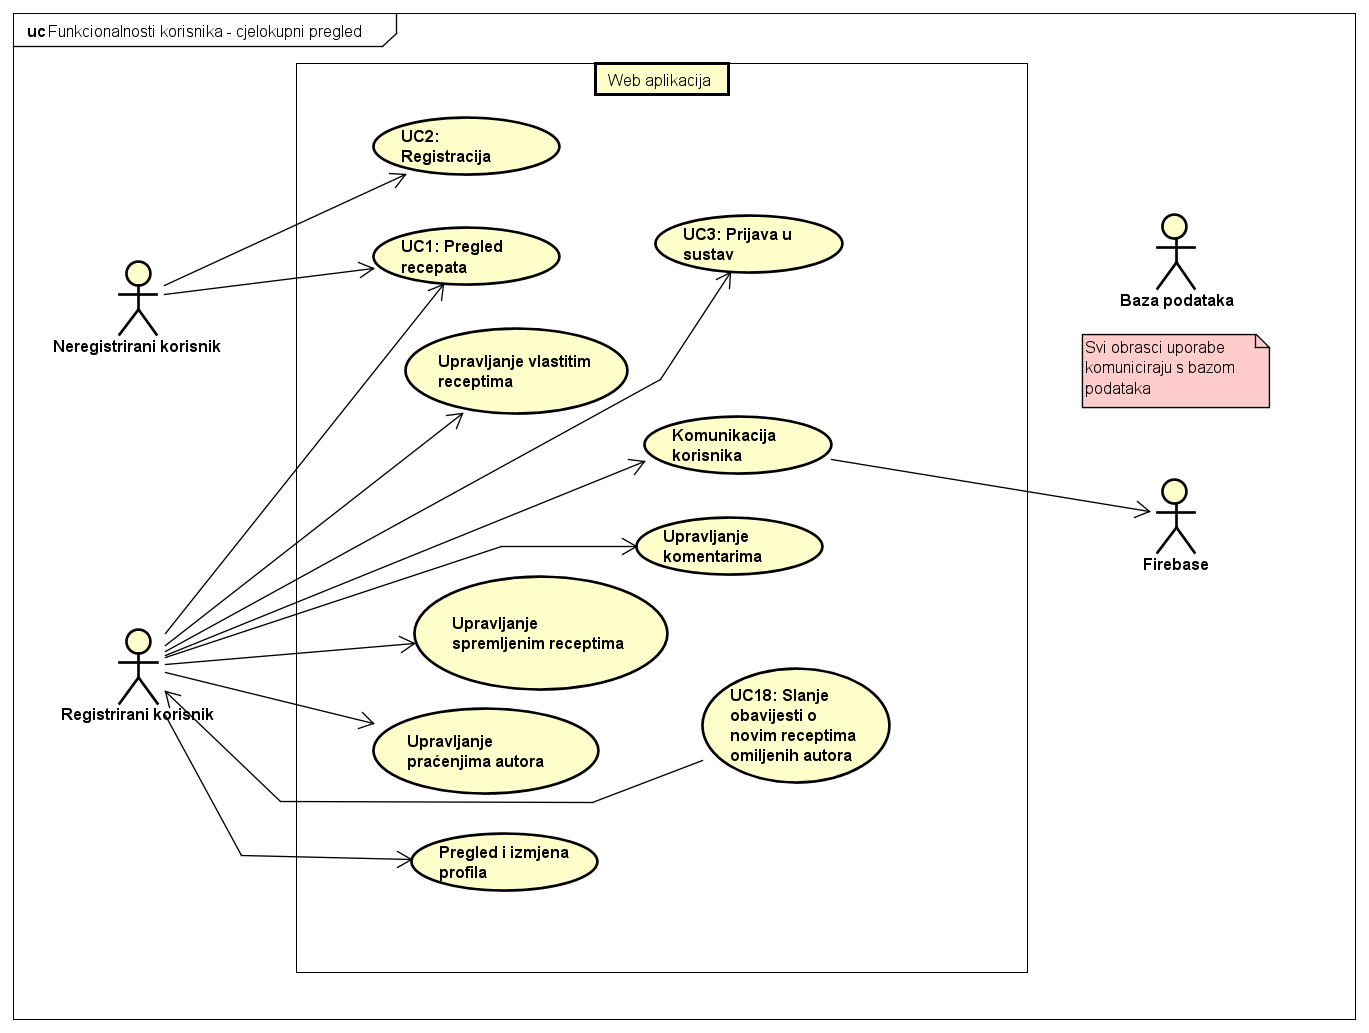
\includegraphics[scale= 0.42]{slike/UseCase Diagram0.png}
						\centering
						\caption{Dijagram obrazaca uporabe, funkcionalnosti korisnika}
						\label{fig:Dijagram obrazaca uporabe, funkcionalnosti korisnika}
					\end{figure}
					\eject
					\begin{figure}[H]
						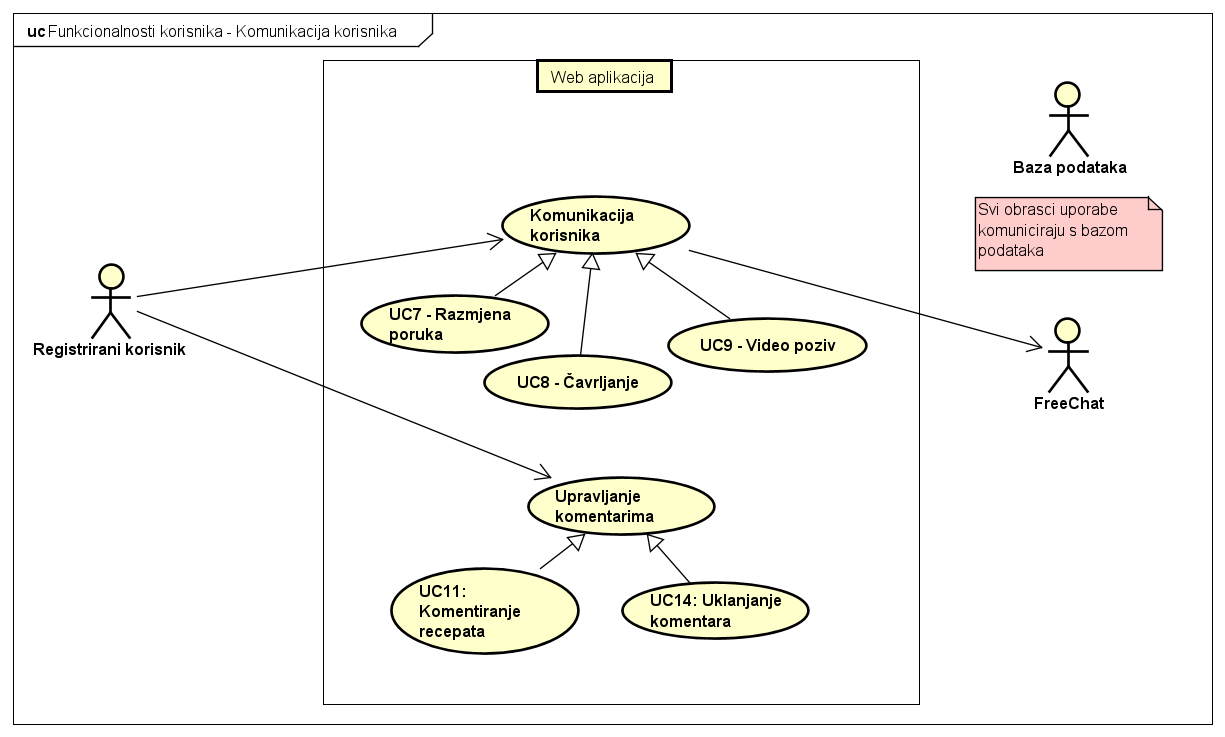
\includegraphics[scale= 0.42]{slike/UseCase Diagram1.png}
						\centering
						\caption{Dijagram obrazaca uporabe, komunikacija korisnika}
						\label{fig:Dijagram obrazaca uporabe, komunikacija korisnika}
					\end{figure}
					\begin{figure}[H]
						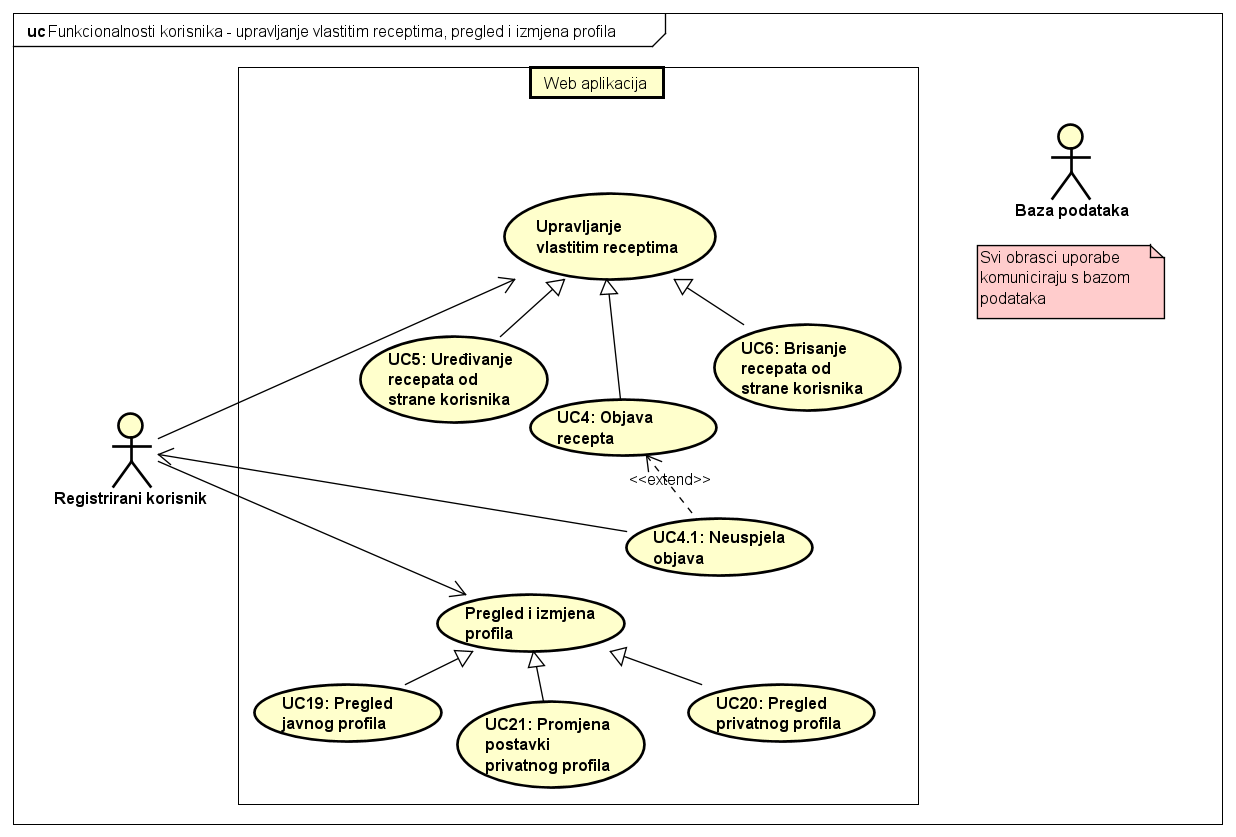
\includegraphics[scale= 0.42]{slike/UseCase Diagram2.png}
						\centering
						\caption{Dijagram obrazaca uporabe, upravljanje receptima, pregled i izmjena profila}
						\label{fig:Dijagram obrazaca uporabe, upravljanje receptima, pregled i izmjena profila}
					\end{figure}
					\begin{figure}[H]
						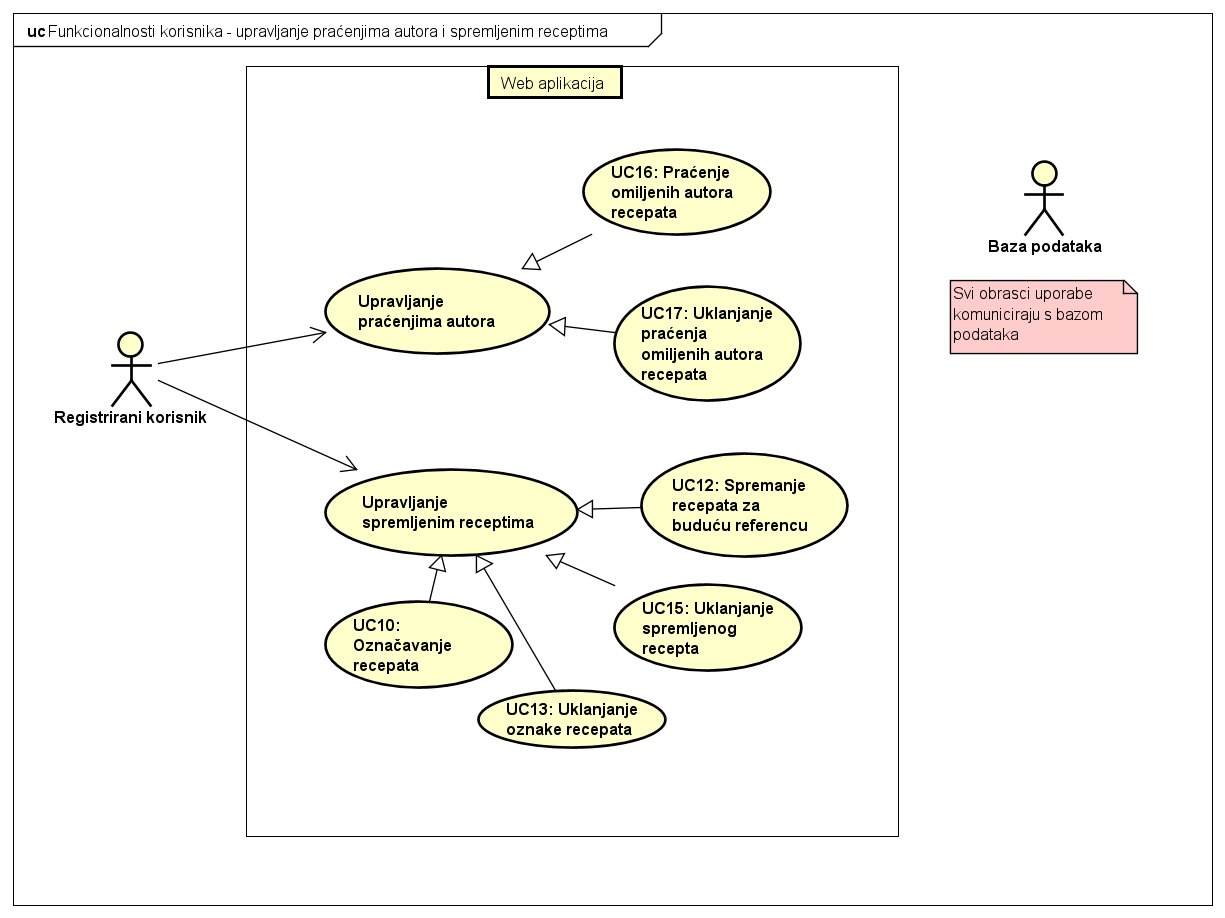
\includegraphics[scale= 0.42]{slike/UseCase Diagram3.png}
						\centering
						\caption{Dijagram obrazaca uporabe, praćenje autora i spremanje recepata}
						\label{fig:Dijagram obrazaca uporabe, praćenje autora i spremanje recepata}
					\end{figure}
					\begin{figure}[H]
						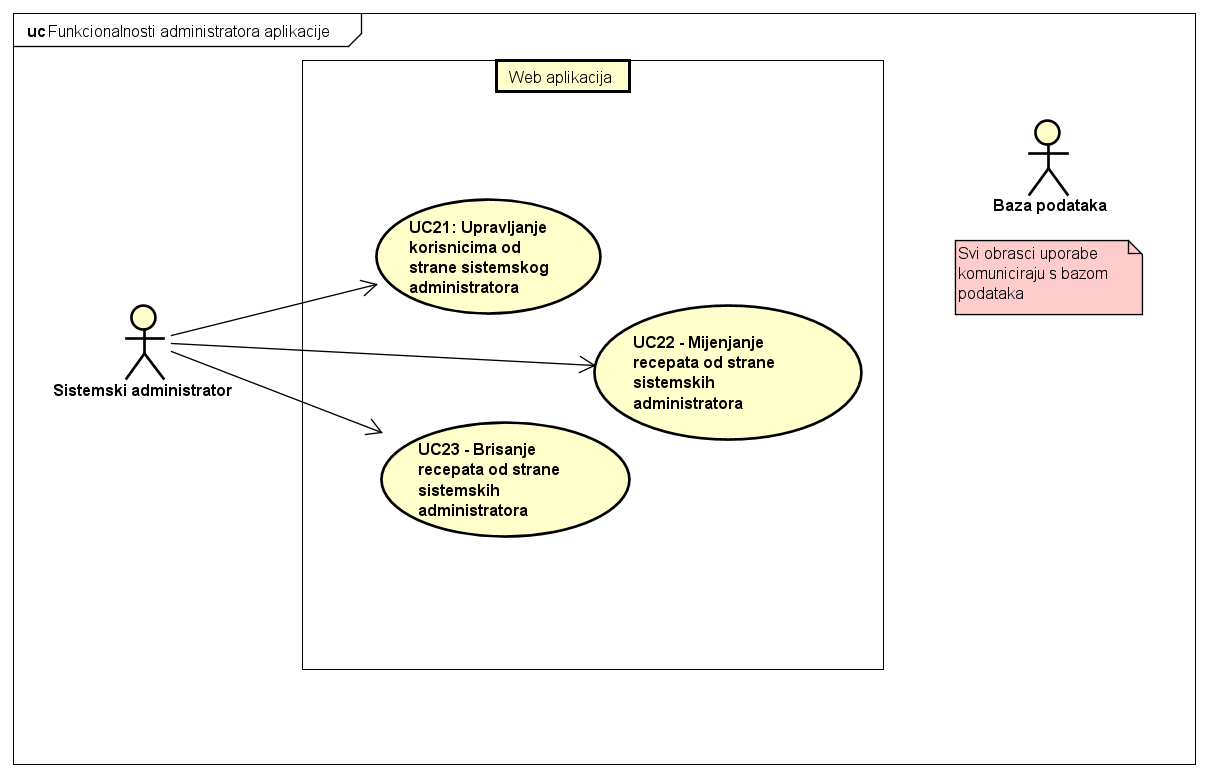
\includegraphics[scale= 0.42]{slike/UseCase Diagram4.png}
						\centering
						\caption{Dijagram obrazaca uporabe, funkcionalnosti administratora}
						\label{fig:Dijagram obrazaca uporabe, funkcionalnosti administratora}
					\end{figure}
					 
				\eject		
				
			\subsection{Sekvencijski dijagrami}
				
				\noindent
				\textbf{Obrazac uporabe UC1-Pregled recepata}\newline
					{Korisnik šalje zahtjev za prikaz recepata po kategorijama, sastojcima i/ili kuhinjama kojim pripadaju. Poslužitelj dohvaća recepete koji zadovoljavaju uvjete i prikazuje ih korisniku. Korisnik sada može spremiti recepte, ako je prijavljen to se provodi, ako nije preusmjeri ga se na stranicu za prijavu.}
				
				
				\begin{figure}[H]
					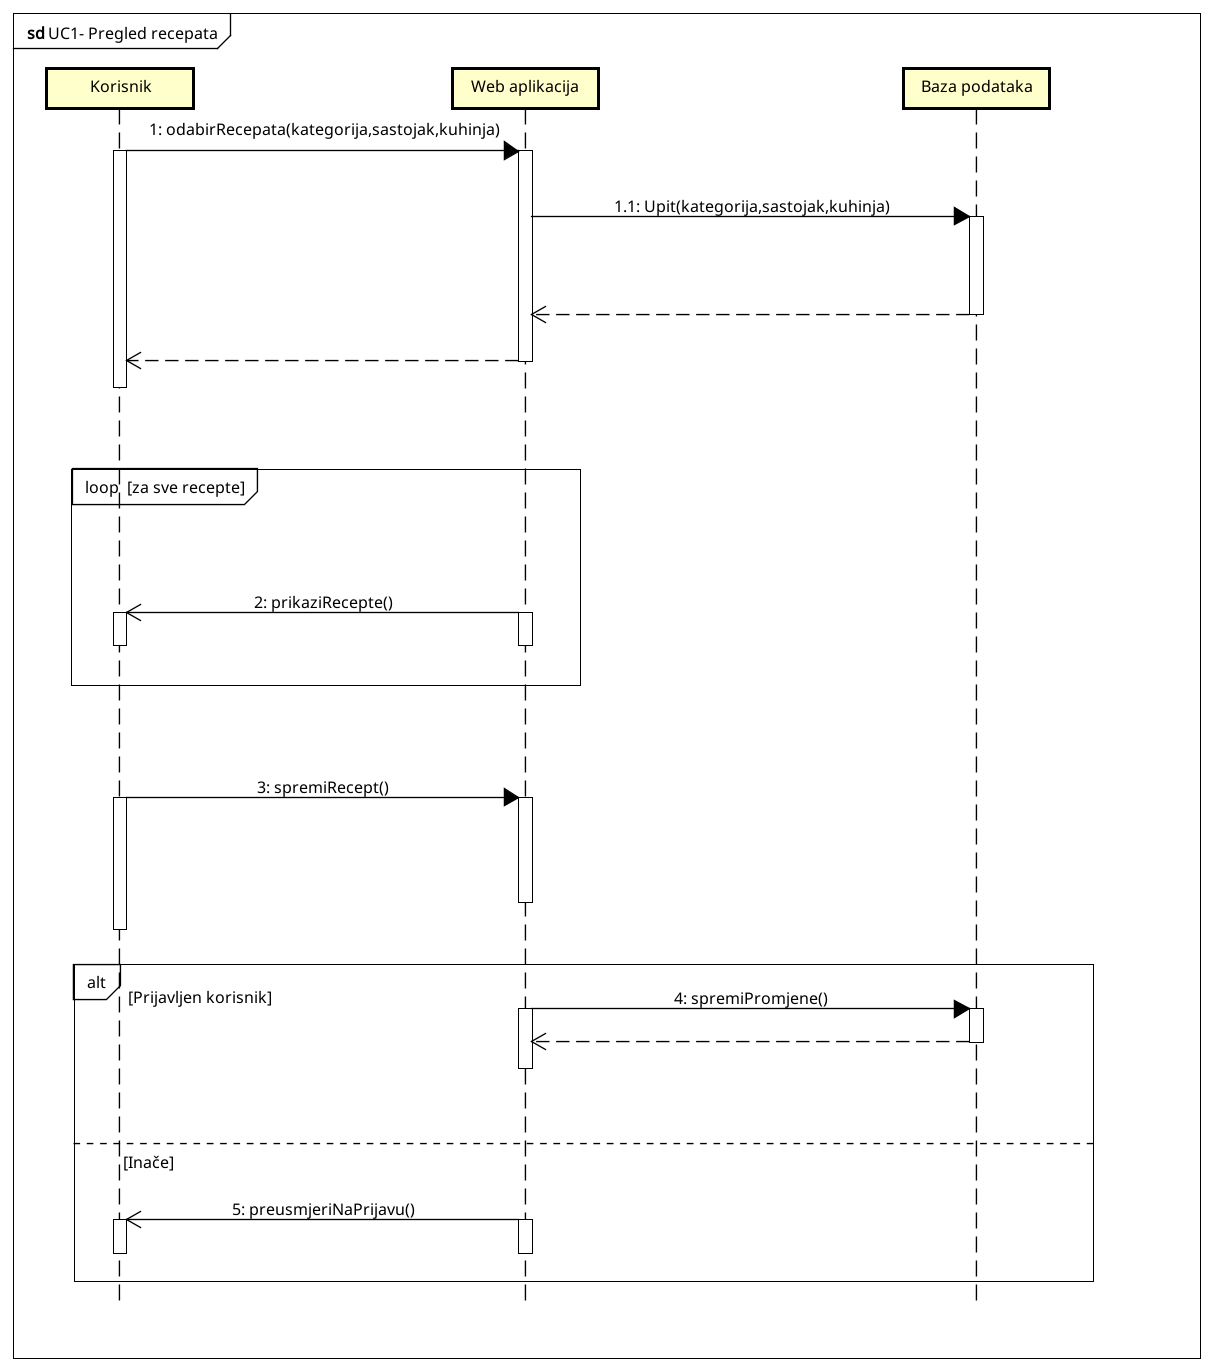
\includegraphics[scale= 0.4]{slike/sekvencijski_dijagramUC1.png}
					\centering
					\caption{Sekvencijski dijagram za UC1}
					\label{fig:Sekvencijski dijagram za UC1}
				\end{figure} 
				\eject

				\noindent
				\textbf{Obrazac uporabe UC3-Registracija}\newline
					{Korisnik se registrira s korisničkim imenom i lozinkom. Ako takav korisnik već postoji, korisniku se ispisuje greška. Inače, korisnik se uspješno registrirao i to se bilježi u bazi podataka.}
				

				\begin{figure}[H]
					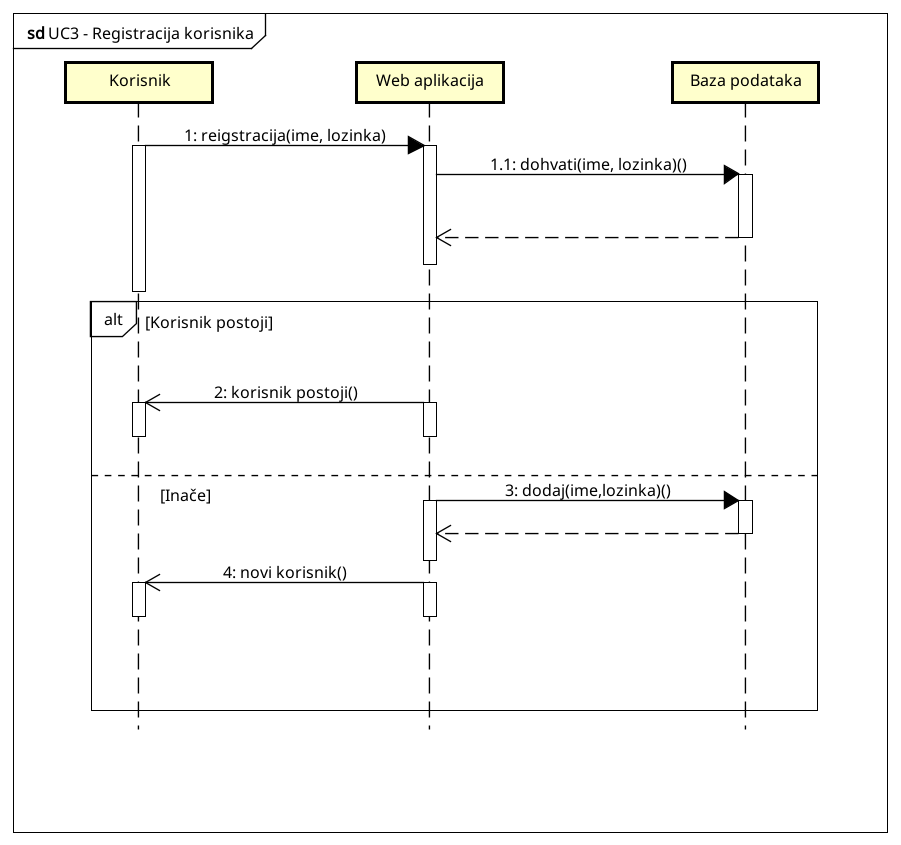
\includegraphics[scale= 0.6]{slike/sekvencijski_dijagramUC3.png}
					\centering
					\caption{Sekvencijski dijagram za UC3}
					\label{fig:Sekvencijski dijagram za UC3}
				\end{figure}
				
				\eject

				\noindent
				\textbf{Obrazac uporabe UC4-Prijava Korisnika}\newline
					{Korisnik pokuša objaviti novi recept. Ako nije prijavljen, preusmjeri ga se na prijavu. Inače, recept se dodaje u bazu podataka i o tome se obavijesti korisnik.}
				

				\begin{figure}[H]
					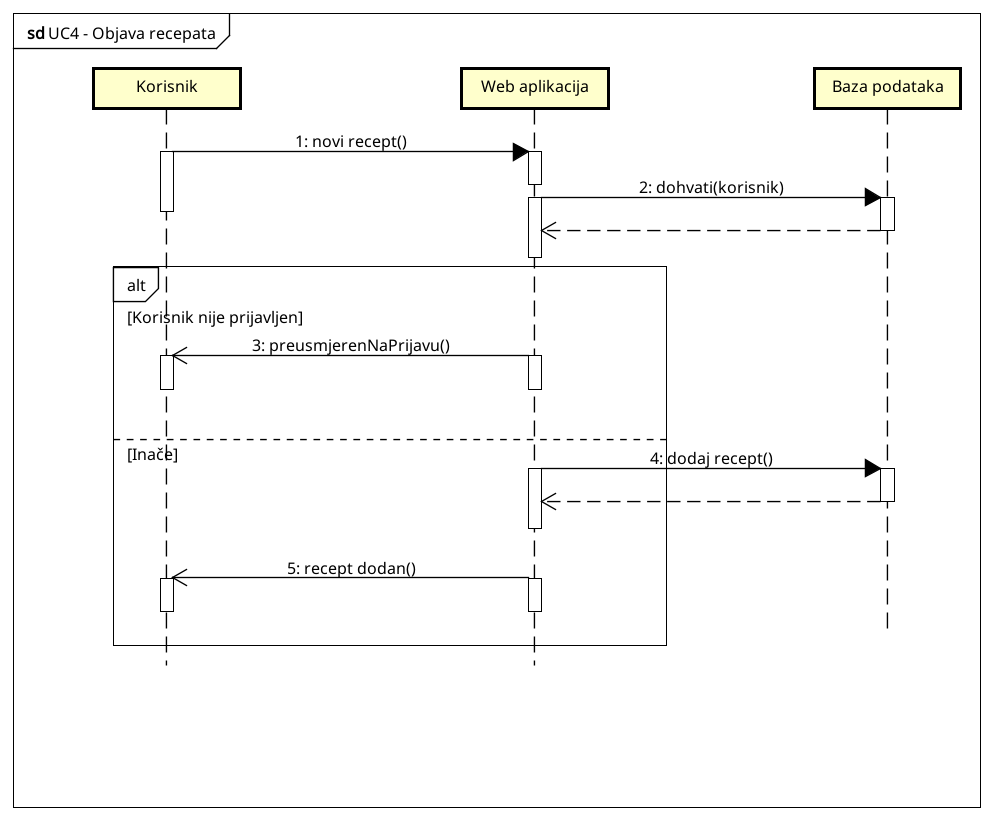
\includegraphics[scale= 0.6]{slike/sekvencijski_dijagramUC4.png}
					\centering
					\caption{Sekvencijski dijagram za UC4}
					\label{fig:Sekvencijski dijagram za UC4}
				\end{figure}

				\eject

				\noindent
				\textbf{Obrazac uporabe UC8-Videopoziv}\newline
					{Korisnik zatraži video poziv s drugim korisnikom. Ako drugi korisnik ne postoji, poziv se ne uspostavlja i o tome se obavijesti prvog korisnika. Inače se šalje zahtjev za video pozivom drugom korisniku, koji ga može odbiti ili prihvatiti. Ako odbije poziv se ne uspostavlja i o tome se obavijesti prvi korsnik. Ako prihvati uspostavi se video poziv između dva korisnika.}
				

				\begin{figure}[H]
					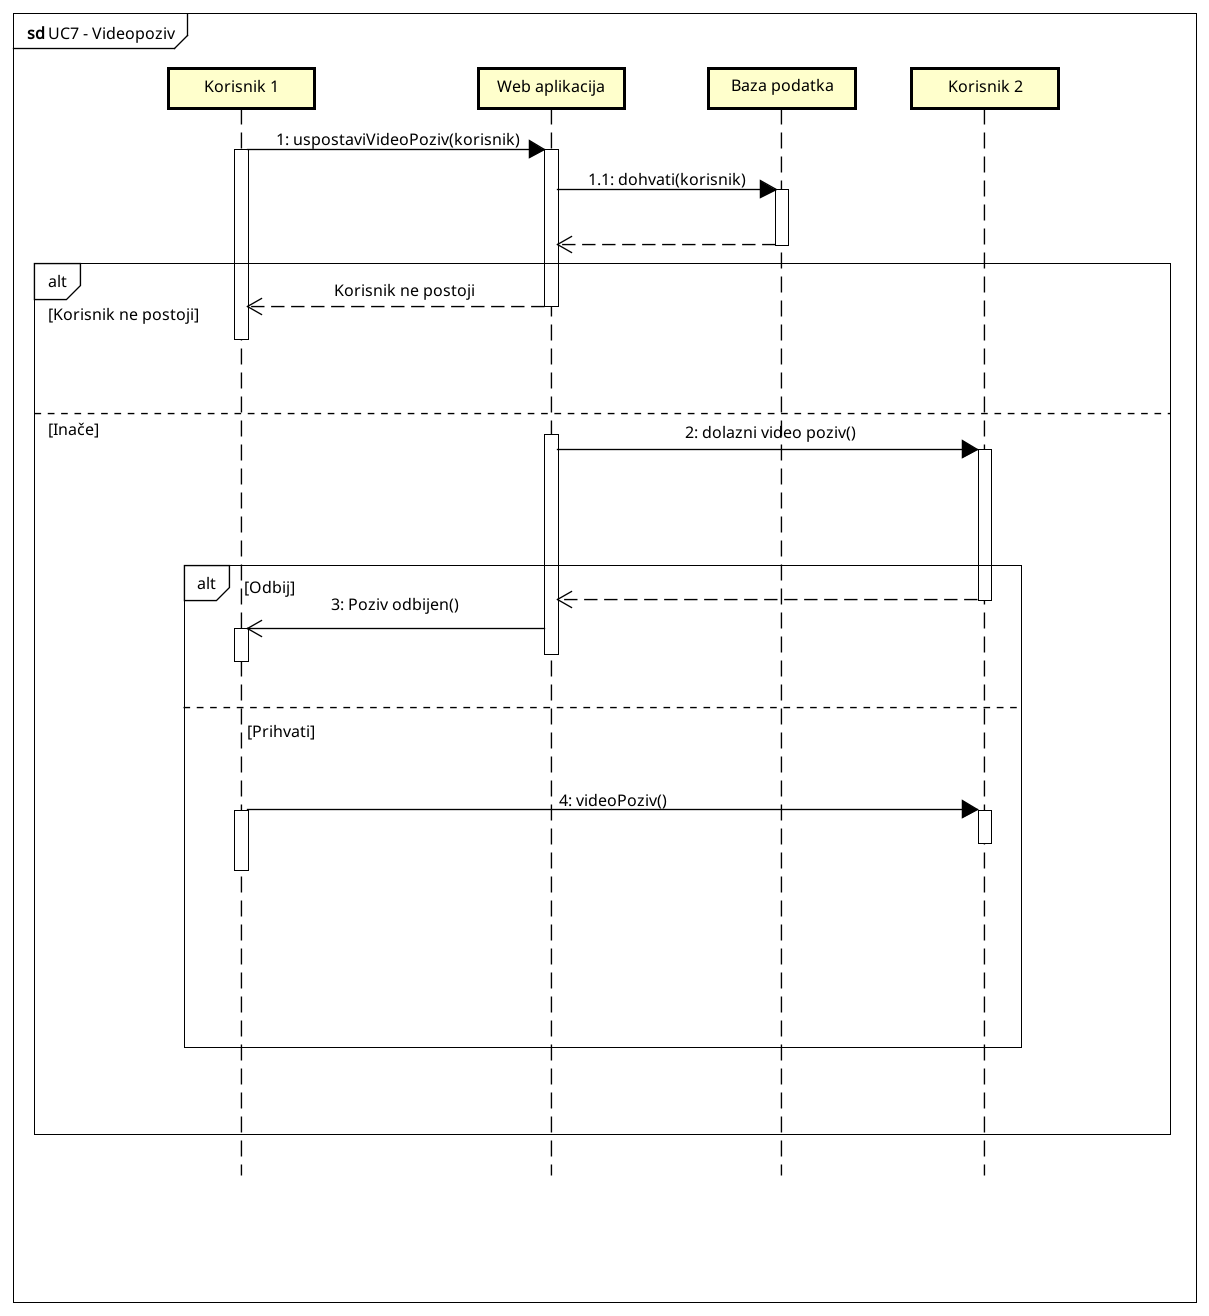
\includegraphics[scale= 0.5]{slike/sekvencijski_dijagramUC7.png}
					\centering
					\caption{Sekvencijski dijagram za UC7}
					\label{fig:Sekvencijski dijagram za UC7}
				\end{figure}
				
				\eject
			
			\section{Ostali zahtjevi}
		
			\textit{Nefunkcionalne zahtjeve koji će se navesti u nastavku teksta pojašnjavaju dodatne zahtjeve koje web aplikacija treba koristiti ili već koristi.}
			
			\begin{packed_item}
				
				\item Sustav treba biti implementiran kao web aplikacija koristeći objektno-orijentirane paradigme i norme kako bi se omogućilo ponovno korištenje dijelova koda/modula.
				\item Nepravilno korištenje web aplikacije ne smije rezultirati padom sustava, odnosno potrebno je usmjeriti korisnika na pravilno korištenje informacionim obavještenjima.
				\item U sustavu treba biti omogućen rad i korištenje web aplikacije od strane više korisnika (cca. 50).
				\item Sustav treba omogućiti komuniciranje korisnika s ostalim korisnicima putem tekstualnog chat-a i video poziva.
				\item Sustav mora podržati dijakritičke znakove hrvatskoj jezika, dakle treba podržati hrvatsku abecedu. Omogućit će se i promjena jezika s hrvatskog na engleski jezik.
				\item Hrvatski jezik je zadani jezik unutar web aplikacije.
				\item Sustav mora imati intuitivno sučelje koje neće stvarati nedoumice kod korisnika odnosno web-aplikacija treba biti jednostavna za korištenje.
				\item Konekcija s bazom podataka mora imati brz odziv. Bilo kakav pokušaj neovlaštenog pristupa informacijama u bazi podataka potrebno je spriječiti i istu adekvatno zašititi.
				\item Web aplikacija koristi proces kripitiranja lozinki za prijavu korisnika koji se tako u hash-ovima spremaju u bazu podataka.
				\item Sustav mora omogućiti korištenje određenih funkcionalnosti samo prijavljenim/registriranim korisnicima.
				\item Učitavanje početne stranice web aplikacije ne smije trajati duže od 5 sekundi.
				\item Pristup sustavu i razmjena podataka se vrši HTTPS protokolom.
				\item Pri razvoju web aplikacije koristi se React Native i Spring framework u Java programskom jeziku.
				
			\end{packed_item}
			 
			 
			 
	